% Name: Linked list
% Description: A singly linked list of four nodes, each holding a value and a pointer to the next, from the head to the null that ends it.
% Tags: linked list, pointers, nodes, data structures

\usetikzlibrary{arrows.meta, calc, positioning, shapes.multipart}

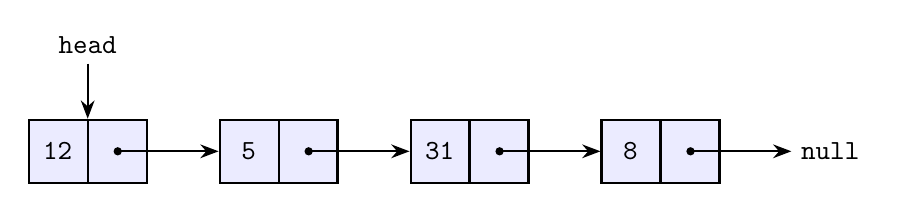
\begin{tikzpicture}[>={Stealth}, node distance=9mm,
    item/.style={rectangle split, rectangle split parts=2, rectangle split horizontal, draw, thick, fill=blue!8, minimum height=8mm, font=\ttfamily, text width=5mm, align=center}]
  \node[item] (n1) {12 \nodepart{two} {}};
  \node[item, right=of n1] (n2) {5 \nodepart{two} {}};
  \node[item, right=of n2] (n3) {31 \nodepart{two} {}};
  \node[item, right=of n3] (n4) {8 \nodepart{two} {}};
  \node[right=of n4, font=\ttfamily] (null) {null};
  % Each pointer starts in the middle of its node's second part.
  \foreach \a/\b in {n1/n2, n2/n3, n3/n4, n4/null} {
    \coordinate (p) at ($(\a.text split)!0.5!(\a.east)$);
    \fill (p) circle (1.5pt);
    \draw[->, thick] (p) -- (\b.west);
  }
  \node[above=7mm of n1, font=\ttfamily] (head) {head};
  \draw[->, thick] (head) -- (n1);
\end{tikzpicture}
